%% LyX 2.4.4 created this file.  For more info, see https://www.lyx.org/.
%% Do not edit unless you really know what you are doing.
\documentclass[english,t]{beamer}
\usepackage{mathptmx}
\usepackage[T1]{fontenc}
\usepackage[latin9]{inputenc}
\usepackage{amssymb}
\usepackage{cancel}

\makeatletter

%%%%%%%%%%%%%%%%%%%%%%%%%%%%%% LyX specific LaTeX commands.
%% Because html converters don't know tabularnewline
\providecommand{\tabularnewline}{\\}

%%%%%%%%%%%%%%%%%%%%%%%%%%%%%% Textclass specific LaTeX commands.
% this default might be overridden by plain title style
\newcommand\makebeamertitle{\frame{\maketitle}}%
% (ERT) argument for the TOC
\AtBeginDocument{%
  \let\origtableofcontents=\tableofcontents
  \def\tableofcontents{\@ifnextchar[{\origtableofcontents}{\gobbletableofcontents}}
  \def\gobbletableofcontents#1{\origtableofcontents}
}

%%%%%%%%%%%%%%%%%%%%%%%%%%%%%% User specified LaTeX commands.
\usetheme{Warsaw}
% or ...

\setbeamercovered{transparent}
% or whatever (possibly just delete it)
\setbeamercovered{invisible} %makes overlays invisible


%gets rid of navigation symbols
\setbeamertemplate{navigation symbols}{}

\usepackage{multicol}

\usepackage{tikz}
\usetikzlibrary{calc}
\usetikzlibrary{plotmarks}
\usepackage{pgfplots}
\pgfplotsset{compat=newest}

\usepackage{calc}
\usepackage[nomessages]{fp}

\usepackage{advdate}    % Advancing/saving dates
\usepackage{datetime}   % Dates formatting
\usepackage{datenumber} % Counters for dates

%\usepackage{pgfpages}
%\pgfpagesuselayout{4 on 1}[a4paper, landscape, border shrink=7mm]
%\pgfpageslogicalpageoptions{1}{border code=\pgfusepath{stroke}}
%\pgfpageslogicalpageoptions{2}{border code=\pgfusepath{stroke}}
%\pgfpageslogicalpageoptions{3}{border code=\pgfusepath{stroke}}
%\pgfpageslogicalpageoptions{4}{border code=\pgfusepath{stroke}}
%%%Don't forget to add 'handout'

\makeatother

\usepackage{babel}
\begin{document}
\newcommand{\xmax}{2000}
\newcommand{\xmin}{0}
\newcommand{\xstep}{0} %must be xmin+n
\newcommand{\ymax}{500}
\newcommand{\ymin}{0}
\newcommand{\ystep}{0} %must be ymin+n

\newcounter{countEx} \setcounter{countEx}{0}
\newcounter{countProb} \setcounter{countProb}{0}
\resetcounteronoverlays{countEx} \resetcounteronoverlays{countProb}

\newcommand{\ex}[3]{
	\addtocounter{countEx}{1}
	\only<#1-#2>{\begin{exampleblock} {Example \chNum.\secNum.\arabic{countEx}.} #3	\end{exampleblock}}
}

\newcommand{\prob}[4]{
	\addtocounter{countProb}{1}
	\only<#1-#2>{\begin{exampleblock} {Problem  \chNum.\secNum.\arabic{countProb}.\,#3} #4	\end{exampleblock}}
}

\newcommand{\yline}[4]{
	(#2 - #4)/(#1 - #3)*(x - #1) + #2
}

\beamerdefaultoverlayspecification{<+->}

%%%%Chapter and Section numbers%%%%%
\newcommand{\chNum}{1}
\newcommand{\secNum}{3}
\newcommand{\secTitle}{The Least Squares Line}

\title[Section \chNum.\secNum: \secTitle]{Section \chNum.\secNum: \secTitle}

\subtitle{Finite Mathematics~~MTH 132~~Spring 2014}

\author{Dr.\,James Ashe}

\titlegraphic{\includegraphics[height=1.5cm]{/home/jim/JamesAshe/JCSU/images/jcsu_bull}}

\institute{Johnson C. Smith University}

\date{{}}

\makebeamertitle 
\begin{frame}{}

Often plotted data lies \emph{close }to a line.
\begin{columns}


\column{5.5cm}

\begin{tabular}{|c|c|}
\hline 
\textbf{Hours } & \textbf{Exam }\tabularnewline
\textbf{Studying} & \textbf{Scores}\tabularnewline
\hline 
2 & 55\tabularnewline
\hline 
4 & 70\tabularnewline
\hline 
5 & 64\tabularnewline
\hline 
6 & 80\tabularnewline
\hline 
9 & 87\tabularnewline
\hline 
\end{tabular}
\begin{itemize}
\item <6->We call this a \emph{linear relation. }
\item <7->But which line?
\item <8->We need a reasonable \emph{approximation. }
\end{itemize}

\column{5.5cm}

\vspace{-.5cm}
%%%%%%%
\begin{tikzpicture} 
\begin{axis}[height=5.5cm, 
	width=5.5cm, axis lines=middle,
	minor x tick num={4},minor y tick num={4},
	grid=both,
	xmin=0,
	xmax=10,
	ymin=50,
	ymax=100,
	xlabel={$Hours$},ylabel={$Scores$}, 
	%xtick={0,50,...,250},%ytick={0,10,20,...,40},%axis line style={-latex},
	every axis/.append style={font=\footnotesize},
	%restrict y to domain=-1:10,%no markers, 
	%every axis x label/.append style={anchor=north},%every axis y label/.append style={anchor=east}
	/pgf/number format/1000 sep={}
	]
  
	\only<2->{\addplot[draw=none,color=blue,solid,mark=*,style={font=\footnotesize}] coordinates {(2,55) (4,70) (5,64) (6,80) (9,87)};}
	
	\only<3->{\addplot[thick,draw=red,domain=0:10]{\yline{2}{55}{6}{80}} node[pos=.65,above] {$$};}
	\only<3->{\addplot[draw=none,color=red,solid,mark=*,style={font=\footnotesize}] coordinates {(2,55)  (6,80)};}

	\only<4->{\addplot[thick,draw=blue,domain=0:10]{\yline{6}{80}{9}{87}} node[pos=.65,above] {$$};}
	\only<4->{\addplot[draw=none,color=blue,solid,mark=*,style={font=\footnotesize}] coordinates {(6,80)  (9,87)};}

	\only<5->{\addplot[thick,draw=purple,domain=0:10]{\yline{4}{70}{9}{87}} node[pos=.65,above] {$$};}
	\only<5->{\addplot[draw=none,color=purple,solid,mark=*,style={font=\footnotesize}] coordinates {(4,70)  (9,87)};}
	
\end{axis}
\end{tikzpicture}
\end{columns}
\end{frame}

\begin{frame}{The Least Squares Line (``best-fit line'')}

\begin{columns}


\column{5.5cm}

\begin{tabular}{|c|c|}
\hline 
\textbf{Hours } & \textbf{Exam }\tabularnewline
\textbf{Studying} & \textbf{Scores}\tabularnewline
\hline 
2 & 55\tabularnewline
\hline 
4 & 70\tabularnewline
\hline 
5 & 64\tabularnewline
\hline 
6 & 80\tabularnewline
\hline 
9 & 87\tabularnewline
\hline 
\end{tabular}

\column{5.5cm}
\begin{block}<2->{Least Square Line \emph{slope}}
$m=\frac{n(\sum xy)-(\sum x)(\sum y)}{n(\sum x^{2})-(\sum x)^{2}}$
\end{block}
\vspace{0cm}
\begin{block}<3->{Least Square Line \emph{y-int}}
$b=\frac{\sum y-m(\sum x)}{n}$
\end{block}
\vspace{0cm}
\begin{block}<4->{Least Square Line}
$y=mx+b$
\end{block}
\end{columns}
\end{frame}

\begin{frame}{}

\begin{columns}


\column{5.5cm}

\begin{tabular}{|c|c|}
\hline 
\textbf{Hours } & \textbf{Exam }\tabularnewline
\textbf{Studying} & \textbf{Scores}\tabularnewline
\hline 
2 & 55\tabularnewline
\hline 
4 & 70\tabularnewline
\hline 
5 & 64\tabularnewline
\hline 
6 & 80\tabularnewline
\hline 
9 & 87\tabularnewline
\hline 
\end{tabular}
\begin{exampleblock}{Equation of the least squares line}
$y=(4.54)x+47.57$
\end{exampleblock}
\begin{block}<2->{Correlation Coefficient}
$r=\frac{n(\sum xy)-(\sum x)(\sum y)}{\sqrt{n(\sum x^{2})-(\sum x)^{2}}\sqrt{n(\sum y^{2})-(\sum y)^{2}}}$
\end{block}


\column{5.5cm}

\vspace{-.5cm}
%%%%%%%
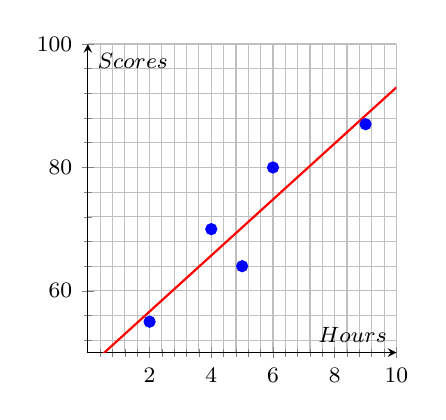
\begin{tikzpicture} 
\begin{axis}[height=5.5cm, 
	width=5.5cm, axis lines=middle,
	minor x tick num={4},minor y tick num={4},
	grid=both,
	xmin=0,
	xmax=10,
	ymin=50,
	ymax=100,
	xlabel={$Hours$},ylabel={$Scores$}, 
	%xtick={0,50,...,250},%ytick={0,10,20,...,40},%axis line style={-latex},
	every axis/.append style={font=\footnotesize},
	%restrict y to domain=-1:10,%no markers, 
	%every axis x label/.append style={anchor=north},%every axis y label/.append style={anchor=east}
	/pgf/number format/1000 sep={}
	]
  
	\only<2->{\addplot[draw=none,color=blue,solid,mark=*,style={font=\footnotesize}] coordinates {(2,55) (4,70) (5,64) (6,80) (9,87)};}
	
	\only<2->{\addplot[thick,draw=red,domain=0:10]{4.54*x+47.57} node[pos=.65,above] {$$};}
	
\end{axis}
\end{tikzpicture}
\end{columns}
\end{frame}

\begin{frame}{}

\prob{1}{}{Find the equation of the least squares line.}{The paired data below consist of the costs of advertising (in thousands) and the number of products sold (in thousands).}

\footnotesize{%
\begin{tabular}{c|c|c|c|c|c|c|c|c}
Cost(\emph{x}) & 9 & 2 & 3 & 4 & 2 & 5 & 9 & 10\tabularnewline
\hline 
Number(\emph{y}) & 85 & 52 & 55 & 68 & 67 & 86 & 83 & 73\tabularnewline
\end{tabular}}

.
\begin{columns}


\column{5.5cm}
\begin{itemize}
\item <3->[]\large$y=2.79x+55.8$
\item <4->[]$r\approx.708$
\end{itemize}

\column{5.5cm}

\vspace{-.5cm}
%%%%%%%
\begin{tikzpicture} 
\begin{axis}[height=5.5cm, 
	width=5.5cm, axis lines=middle,
	minor x tick num={4},minor y tick num={4},
	grid=both,
	xmin=0,
	xmax=11,
	ymin=50,
	ymax=90,
	xlabel={$Cost$},ylabel={$Number$}, 
	%xtick={0,50,...,250},%ytick={0,10,20,...,40},%axis line style={-latex},
	every axis/.append style={font=\footnotesize},
	%restrict y to domain=-1:10,%no markers, 
	%every axis x label/.append style={anchor=north},%every axis y label/.append style={anchor=east}
	/pgf/number format/1000 sep={}
	]
  
	\only<2->{\addplot[draw=none,color=blue,solid,mark=*,style={font=\footnotesize}] coordinates {(9,85) (2,52) (3,55) (4,68) (2,67) (5,86) (9,85) (10,73)};}
	\only<3->{\addplot[thick,draw=red,domain=0:11]{2.79*x+55.8} node[pos=.65,above] {$$};}
	

\end{axis}
\end{tikzpicture}
\end{columns}
\end{frame}

\end{document}
